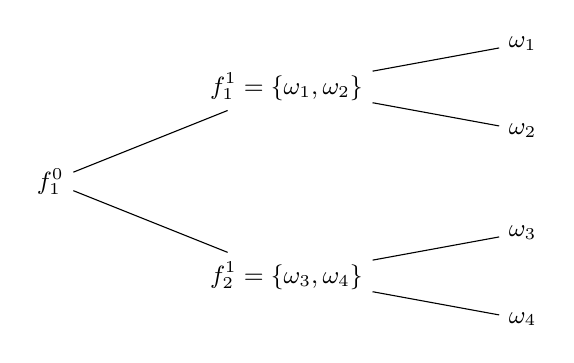
\begin{tikzpicture}[grow=right,level 1/.style={level distance=3cm,sibling distance=2.4cm},level 2/.style={level distance=3cm,sibling distance=1.1cm},every node/.style={font=\small}]
\node{$f^0_1$}
 child{node{$f^1_2=\{\omega_3,\omega_4\}$} child{node{$\omega_4$}} child{node{$\omega_3$}}}
 child{node{$f^1_1=\{\omega_1,\omega_2\}$} child{node{$\omega_2$}} child{node{$\omega_1$}}};
\end{tikzpicture}
